\documentclass[12pt, titlepage=true, toc=bib]{scrartcl}


%Deutsche Silbentrennung
%Trennung von Wörtern mit Umlauten
%Deutsche Sprachregeln
\usepackage[utf8]{inputenc}
\usepackage[T1]{fontenc}
\usepackage[english]{babel}

%Schriftart
\usepackage[bitstream-charter]{mathdesign}
\usepackage[activate={true, nocompatibility}, final, tracking=true, kerning=true, spacing=true, factor=1100, stretch=10, shrink=10]{microtype}
%Selbe Schriftart für Überschriften												
\addtokomafont{disposition}{\normalfont\bfseries}

\usepackage{amsmath}

%Zeilenabstand							
\usepackage[onehalfspacing]{setspace}

%Literaturverwaltung
\usepackage[backend=biber, style=authoryear, date=year, doi=false, isbn=false, url=false, maxcitenames=2, maxbibnames=8]{biblatex}		
%Formatierung für Anführungszeichen
\usepackage[autostyle]{csquotes}
%u.a. in et al. umwandeln
\DefineBibliographyStrings{ngerman}{andothers = {{et\,al\adddot}},}
%Formatiert die Zitationsklammern
\renewcommand{\labelnamepunct}{\addcolon\addspace}
\renewcommand{\postnotedelim}{\addcolon\addspace}
\DeclareFieldFormat{postnote}{#1}
\DeclareFieldFormat{multipostnote}{#1}
%Leerzeile zwischen den Einträgen im Literaturverzeichnis
\setlength{\bibitemsep}{0.5\baselineskip plus 0.5\baselineskip}
%Schrägstrich bei zwei Autor*innen
\renewcommand{\multinamedelim}[0]{/}
\renewcommand{\finalnamedelim}[0]{/}
%URL bei Artikel- und Büchereinträgen entfernen
\DeclareSourcemap{
  \maps[datatype=bibtex]{
    \map{
      \pertype{article}
      \pertype{book}
       \step[fieldset=url, null]
    }
  }
}


\addbibresource{HA_SNA.bib}

%Seitenränder
%\usepackage[right=4	cm,]{geometry}

%Paket, um Grafiken einzubinden
\usepackage{graphicx}
%\usepackage{float}
%Paket, um Grafiken davon abzuhalten, außerhalb bestimmter grenzen zu floaten [section]: verbietet gleiten außerhalb der Section
%\usepackage[section]{placeins}
%zum Formatieren der Bildunterschriften
\usepackage{caption}
\captionsetup{format=plain, indention=0cm, justification=justified, singlelinecheck=off, width=.95\linewidth, font={small, singlespacing}}
%\captionsetup[table]{name=Tab. }
\setkomafont{captionlabel}{\bfseries}

%Wird für das r-Paket stargazer benötigt
\usepackage{dcolumn}

%Listen
%\usepackage{enumitem}

%pdf-Dateien einbinden
%\usepackage{pdfpages}

%Anhang ohne Seitenzahl im ToC
%\makeatletter
%\let\partbackup\l@part
%\renewcommand*\l@part[2]{\partbackup{#1}{}}
%\makeatother

%\clubpenalty = 10000
%\widowpenalty = 10000
%\displaywidowpenalty = 10000

%Verlinktes ToC
\usepackage[colorlinks, pdfpagelabels, pdfstartview=FitH, bookmarksopen=true, bookmarksnumbered=true, linkcolor=black, urlcolor=black, plainpages=false, hypertexnames=false, citecolor=black]{hyperref}



\begin{document}

\titlehead{\flushleft{University of Copenhagen\\
			Department of Political Science\\
			Social Network Analysis (ASTK18106U)\\
			Yevgeniy Golovchenko
			}}
\author{Ole Fechner, Johannes Kopf}
\title{Structure and Strategy of the Internet Research Agency on Twitter}


\date{\normalsize{Copenhagen, \today}}

\publishers{\flushleft{\normalsize{Boddinstr. 15\hfill Moselstr. 50\\
							 12053 Berlin\hfill 50674 Cologne\\
							 ole.fechner@fu-berlin.de\hfill jkopf@posteo.de\\
							 MA Political Science\hfill MA Political Science}}}

\maketitle[0]

\newpage

\thispagestyle{empty}
\tableofcontents

\newpage

\thispagestyle{empty}
\listoftables

\newpage

\thispagestyle{empty}
\listoffigures

\newpage
\setcounter{page}{1}

\section{Introduction}

``Frankly, the United States is under attack'', said Dan Coats, director of U.S. National Intelligence in an interview about the influence of Russian troll accounts in the 2016 U.S. presidential elections. (cite NBC artikel). What seems to be a drastic statement has been emphasized by Twitter committing a list of 2,857 supposedly Russian troll accounts connected to the state-sponsored Internet Research Agency (IRA) to U.S. Congress. (cite twitter-doc), who have been active on Twitter for much longer than the 2016 elections. Coats expects Russia ``to continue using propaganda, sympathetic spokesmen, and other means of influence to [...] exacerbate social and political fissures in the United States'' (cite NBC artikel). With its low costs, low risk and the difficulties of tracing it back, Twitter appears especially attractive as an instrument for gaining influence in foreign countries. The degree of professionalism should thereby not be underestimated, with division in day and night shifts, training in English grammar pr US holidays and quotas to meet to monitor the activity of the troll workers. \citep{kirby_what_2018}. This suggests an intentional strategy of troll behaviour, an orchestrated act of state-institutional interference with a foreign election that urges for research on the matter. Given this relevance of the matter, research on the activity of Twitter trolls suggests shedding some light on an issue of growing importance for everyday politics.

With the recency of the IRA's discovery, only few researchers have approached the topic and actually published their results. (e.g. see \citep{golovchenko_state_2018} for an analysis of Twitter information warfare over Ukraine, or  \citep{stewart_examining_2018} for an analysis of trolls and polarization in a retweet network). Linvill/Warren \citep*{linvill_troll_2018} present and early analysis using a sequential mixed method design, first qualitatively categorizing the Twitter accounts into groups as for example left or right troll and subsequently examining those account's activity over time. This paper seeks to build upon Linvill and Warren's work by further investigating potential differences in troll behavior between various communities of trolls. As a research question, we want to ask, how does IRA troll account behavior differ between the Twitter communities they engage in? As a theoretical foundation, we rely on the concepts of agenda-building and astroturfing, assuming strategic activity and behavior of Russian trolls in trying to gain influence on Twitter. We are using dataset of 147,428 retweets by 453 trolls, which includes a large share of trolls who have been qualitatively categorized by Linvill/Warren (2018). We are applying methods of Social Network Analysis (SNA), building a ego-centered retweet network using retweets as ties between different Twitter accounts as nodes. First, we are running community detection algorithms to cross-validate Linvill and Warren's \citep*{linvill_troll_2018} findings. We find that there is a sufficiently good fit of the detected communities with the qualitative categories. Secondly, we analyze the graph densities in the different communities finding strong differences between communities. Third, we are computing out- and indegrees for our nodes, again finding support for different behavior across communities of Twitter accounts. As a last measure, we are computing different k-cores, finding an overall most active and inter-connected community of right trolls. We then discuss the findings with a focus on the mechanics of information spreading and the limitations of our SNA approach with regard to the network being ego-centered.


\section{Agenda-building and Astroturfing}

The process of trying to move an actors agenda to the agenda of other actor's, especially policymakers, is defined as \textit{agenda-building} (\cite[3]{linvill_troll_2018}). This can also be extended to the question of how the public views certain issues, usually by analyzing media coverage of those issues: ``Agenda-building research examines how certain groups, such as those in politics and business, influence what issues journalists cover as well as how the public views issues'' (\cite[434]{parmelee_agenda-building_2014}). Since the rise of social media platforms like Twitter and Facebook, agenda-building takes place in those environments. This is due to journalists drawing heavily on Twitter for their job and, on the other hand, research shows that Twitter is the most popular social media platform for participating in political discussions, which from there are often taken to other media (\cite[435, 437]{parmelee_agenda-building_2014}). Influencing the citizens of another country through the use of media is nothing new, rather it is used in conflicts or during war regularly. ``However, Russia's work on social media has taken agenda-building efforts by nations into a new context'' (\cite[3]{linvill_troll_2018}).

Closely linked to agenda-building is a second phenomenon called (political or/and online) \textit{astroturfing}, which can be characterized as the ``creation of a false or exaggerated impression of grassroots support'' (\cite{harcup_astroturfing_2014}). It describes the strategic and coordinated approach of a group with the aim to create the impression of a certain public opinion, that might not exist in that way. On social media, those groups use many different accounts that post and interact with regular users to create the desired impression. For the purpose of this paper, we see astroturfing as a strategy of agenda-building. The anonymity provided by platforms like Twitter, as well as the covert structure of those groups, make them very hard to discover (\cite[564]{yang_how_2017}). This exploratory study will therefore take the structure of the IRA as a staring point, instead of the presumed agenda behind the organization. Social Network Analysis, which will be introduced in the next section, offers an excellent tool box to conduct this task.


\section{The Social Network Analysis}

To analyze the structure and possible strategies of the IRA, we will take Social Network Analysis (SNA) as the method of choice. The data-driven character of SNA -- the notion of people relating to each other, and the significance put into the structure and strength of those relations being almost the only one (\cite[982]{golovchenko_state_2018}) -- makes it especially viable for our exploratory approach. SNA conceptualizes the linkages between actors as \enquote{channels for transfer or \enquote{flow} of resources}, while the actors themselves are seen as ``interdependent rather than independent, autonomous units'' (\cite[4]{wasserman_social_1994}). Therefore, the different actor attributes are seen as emerging out of their relations and not vice versa, as in most other types of quantitative analyses (\cite[8]{wasserman_social_1994}). This allows us to ignore the question of the actual people behind different accounts and tell something about the IRA and its structure, as well as its strategy, as a whole. The most important relation to analyze how the IRA uses astroturfing as a strategy for agenda-building is the distribution of information, in this case via retweets. Accordingly, the foundation of this paper will be a social network consisting of Twitter accounts as nodes and retweets as edges (or linkages).


\subsection{Data: An ego-centered retweet network}

We will use a dataset, published by NBC News (\cite*{popken_twitter_2018}), consisting of 203,451 Tweets by 453 accounts between July 2014 and September 2017, which were linked to the IRA by an official document handed over to US Congress by Twitter. Twitter justifies this linking by referring to ``third party sources'', which makes it impossible to reconstruct or evaluate their method. Therefore, we have to assume those accounts' links to the IRA to be correct, as it is the best evaluation available.

To create the social network, we need to clean the data: First, we drop any of the tweets that are not retweets, which leaves us with 147,428 retweets by 453 troll accounts. Second, 120 trolls, who did not retweet at all, were dropped accordingly. Our dataset now consists a set of 333 unique troll Twitter handles\footnote{A Twitter handle is the screen name of a Twitter account that can be changed by the users.}, who are retweeting others. A variable stating the unique User ID is used to validate uniqueness of the users, showing that there are indeed no duplicate User IDs in the dataset. Since, we only have information about who these 333 accounts did retweet, but not by whom they were retweeted, the network is ego-centered around the group of 333 trolls. Of these 333 trolls, 151 (ca 45\%) retweeted others and were themselves retweeted by other trolls, thus being both sender and receiver. 182 (ca 55\%) trolls only retweeted others, but were not retweeted themselves, making them only senders.\footnote{We define a retweet sender as the person retweeting an original Tweet by another person, who, accordingly, is the retweet receiver.} A third group of 71 trolls was found by looking at who was retweeted by the original group of trolls in the data, thus increasing the number of trolls in our data to a group of 404. These 71 trolls were retweeted by others, though did not send retweets themselves. Finally, the big body of users in the dataset consists of 36,485 users, who are retweeted by the trolls, but are not themselves categorized as trolls by Twitter. Table~\ref{tab:userstat} gives a first overview over out dataset. Overall, there are 36,889 unique twitter users in the dataset, 404 classified trolls and 36,485 non-trolls. The retweets contain relational information about one user retweeting another, therefore creating a directional edge between the two. Thus, the graph is a directed, ego-centered network of 404 IRA accounts with 36,889 unique Twitter accounts as nodes and edges representing retweets from the sender to the receiver.

\begin{table}[!ht] \centering 
\begin{tabular*}{.95\linewidth}{@{\extracolsep{\fill}} lrrr} 
\\[-1.8ex]\hline 
\hline \\[-1.8ex] 
User & N & Senders & Receivers \\ 
\hline \\[-1.8ex] 
Troll & 404 & 333 & 222 \\ 
Non-Troll & 36,485 & 0 & 36,485 \\ 
Total & 36,889 & 333 & 36,707 \\ 
\hline \\[-1.8ex] 
\end{tabular*} 
  \caption[User Statistics]{Distribution of troll accounts and retweet sender and receiver in the data.}
  \label{tab:userstat} 
\end{table} 

To further extend our data and our scope of analysis, we are adding additional qualitative information on the IRA trolls, provided by Darren Linvill and Patrick Lee Warren (\cite*{linvill_troll_2018}) via the online news outlet FiveThirtyEight (citation). Linvill and Warren conduct a qualitative analysis, categorizing a sample of 1,133 IRA troll accounts by examining the tweet content and the account names, applying a temporal analysis of the trolls tweeting behavior after. They ``identified five categories of IRA-associated Twitter handles, each with unique patterns of behaviors: \textit{Right Troll}, \textit{Left Troll}, \textit{Newsfeed}, \textit{Hashtag Gamer}, and \textit{Fearmonger}.'' (\cite[6]{linvill_troll_2018}). In addition, there are three categories, which are not used within their analysis, those being \textit{Non-English}, \textit{Commercial} and \textit{Unknown}. The categories \textit{Right Troll} and \textit{Left Troll} need little explanation, as they include users who broadcasted right-leaning populist and socially liberal messages. \textit{Hashtag Gamers} are users who are playing word games on Twitter, mostly non-political, though sometimes including left- or right-leaning messages. \textit{Newsfeed} Trolls are posing as local US News Agencies, mostly linking to legitimate news content, often with a pro-Russian perspective. Fearmongers spread news of crisis events such as Tweets about salmonella infections. The \textit{Non-English} troll category includes users who tweeted in other languages than English, predominately Russian, some German and little French and Spanish. \textit{Commercial} Trolls are not included in our dataset. Finally, users were categorized as \textit{Unknown}, if they could not be assigned to other categories for lack of information in their tweets. These categories will be included in this paper's analysis, since might be interesting to see how they interact with the other trolls. We are appending Linvill and Warren's account categories to our data, finding categories are available for 394 of the 404 troll handles in our dataset, meaning that around 98\% of the trolls in our dataset are categorized. Table~\ref{tab:trollstat} shows the distribution of the categories among our dataset.

\begin{table}[!ht] \centering 
\begin{tabular*}{.95\linewidth}{@{\extracolsep{\fill}} lrrrr} 
\\[-1.8ex]\hline 
\hline \\[-1.8ex] 
Category & N & Senders & Receivers & Average followers \\ 
\hline \\[-1.8ex] 
Right & 101 & 75 & 90 & 4649 \\ 
Left & 110 & 104 & 48 & 1783 \\ 
Hashtag Gamer & 61 & 43 & 60 & 3021 \\ 
Non-English & 106 & 100 & 7 & 2127 \\ 
Newsfeed & 11 & 1 & 10 & 16446 \\ 
Fearmonger & 4 & 0 & 4 & 0 \\ 
Unknown & 11 & 10 & 3 & 3306 \\ 
Total & 404 & 333 & 222 & 4476 \\ 
\hline \\[-1.8ex] 
\end{tabular*} 
  \caption[Troll Statistics]{Distribution of account types categorized by Linvill and Warren (2018)}
  \label{tab:trollstat} 
\end{table} 
 
As another attribute, we are appending information on the count of followers of the troll accounts from a second dataset provided by NBC news. The information on the count of followers provided only includes one figure and does not vary over time, without specification of when these follower counts were obtained. We will assume that they are at least to some degree representative and use them as a heuristic. Table~\ref{tab:trollstat} gives the average number of followers for each account category. Finally, we are using the full time period of retweets, from July 2014 to September 2017. This paper is not interested in a time period preceding a specific event, like an election or a specific trending discussion, but rather strategic behavior of the trolls in general. That is why it seems to be the right approach to include all of the Tweets in the analysis.


\subsection{Methods}

To understand the IRA's division of labor between the accounts, we begin with testing weather Linvill and Warren's qualitative findings of the different account types would be reproducible via using network properties. For this, we will draw on a community detection algorithm based on modularity, known as the Louvain Method (\cite{blondel_fast_2008}).\footnote{For our network, this algorithm produced the best results. The Infomap algorithm (\cite[cf.][]{rosvall_maps_2008}) results in one big community containing ca 98\% of the nodes.} Communities are mesoscopic structures of a graph, that consist ``of a group of nodes that are relatively densely connected to each other but sparsely connected to other dense groups in the network'' (\cite[1083]{porter_communities_2009}). The Louvain algorithm is based on modularity, ``a scalar value between -1 and 1 that measures the density of links inside communities as compared to links between communities'' (\cites[2]{blondel_fast_2008}[cf. also][1089]{porter_communities_2009}). It approximately maximizes the modularity for each node, thus identifying communities. Finally we will compare the communities with Linvill and Warren's account types, to see weather we can better understand the identified community structure.

One important measure for the cooperation of the accounts is graph density, the proportion of all possible edges that are present in the graph (\cite[101]{wasserman_social_1994}). Since the network is ego-centered, it only makes sense to calculate density for the troll subgraph. We will then compare densities of the different communities, which can give an indication weather the IRA has distinctive strategies for those groups. Following Wassermann and Faust (\cite*[102]{wasserman_social_1994}) we calculate the density of the different community subgraphs \( \Delta_{c} \) as: \[ \Delta_{c} = \frac{2L_{c}}{g_{c}(g_{c} - 1)} ,\] where \( L_{c} \) is the number of edges present in the community subgraph, and \( g_{s} \) is the number of nodes in said graph. In communities with higher density, the accounts are working more together, meaning they spread information further through retweeting, while accounts in less dense communities rely more on information they put into the network themselves.

Identifying the most important accounts helps to understand the structure of the IRA. Operationalizing importance in SNA is usually done through centrality and prestige indices, whereas not only the chosen actors are considered prestigious, but also those doing the choosing (\cite[170]{wasserman_social_1994}). Since the network is ego-centered around the troll accounts, the indices have limited reach in their interpretation, but still deliver important insights. To show the most central accounts, we will calculate outdegree. The index can only be computed for IRA accounts, since they are the only retweeting in our dataset. We will calculate the outdegree weighted and unweighted respectively, the former results in the accounts that retweet the majority of different accounts, the latter in those retweeting the most.\footnote{A weighted graph is a graph in which each edge carries a value (\cite[140]{wasserman_social_1994}), in this case the number of retweets between two accounts. In an unweighted graph, each edge has the value 1.} The outdegree of a node \( d_{out}(n_{i}) \) is computed as \[ d_{out}(n_{i}) = \sum_{j} x_{ij} ,\] where \( x_{ij} \)\footnote{Note that in- and outdegree are calculated for directed graphs, hence \( x_{ij} \neq x_{ji} \).} is an edge from \( i \) to \( j \) (\cite[cf.][178]{wasserman_social_1994}. For the weighted outdegree \( x_{ij} \) is multiplied by the value of the edge. Prestige, on the other hand, will be calculated through indegree, which results in those accounts retweeted the most and can therefore tell about what accounts the IRA draws on. It will also be computed for the weighted and unweighted graph separately, which shows the accounts retweeted by the majority of different accounts and those retweeted the most in general respectively. The indegree of a node \( d_{in}(n_{i}) \) is computed simply as \[ d_{in}(n_{i}) = \sum_{j} x_{ji} ,\] where \( x_{ji} \) is an edge from \( j \) to \( i \) (\cite[cf.][202]{wasserman_social_1994}). For the weighted outdegree \( x_{ji} \) is multiplied by the value of the edge.

Finally, we will look at the most engaged users in the network to identify the so-called super-spreaders of information. In SNA, the ability to spread information better than other individuals is ascribed to their unique location in the network, which makes identifying those a prime task of analyzing networks used for false information (\cite[1]{pei_searching_2015}). Pei et al. (\cite*{pei_searching_2015}) show that, compared to other approaches, the k-core method predicts the super-spreaders most accurately. \enquote{A k-core is a maximal subset of the network where all nodes are connected to at least \enquote{k} number of other nodes: so \enquote{k} can be any whole number} (\cite[983]{golovchenko_state_2018}). Hence, the k-core specifies a subgraph via the number of ties that must be present between nodes, it is based on the nodal degree. We can define a subgraph \( G_{s} \) as a k-core if \[ d_{s}(i) \geq k \text{ for all } n_{i} \in N_{s} ,\] where \( d_{s}(i) \) is the (in-)degree of node \( i \) and \( N_{s} \) the set of nodes in the subgraph (\cite[266]{wasserman_social_1994}). Once again, the network being ego-centered limits the validity of the results, since every non-troll in reality has a higher degree through retweets from other non-troll accounts and retweeting themselves. We can therefore only identify the most important IRA accounts regarding their own network. To account for this, we will also compute the k-in-core through the indegrees. The idea is that information from one account is spread quickly, if this account is retweeted a lot and the accounts retweeting it also get retweeted a lot.


\section{Analyzing the IRA Retweet Network}

In the preceding chapter, the data and methods that form the basis of our analysis have been introduced. Figure~\ref{fig:graph} shows the entire retweet network consisting of three main clusters. We will focus our analysis on those clusters in four steps. First, the results of the modularity community detection algorithm are illustrated and new communities are established, based on our findings, as well as the qualitative coding of Linvill and Warren. Second, graph densities are compared between these communities. Third, degree centrality indices are analyzed for the whole graph to identify the most active IRA accounts and the most prestigious accounts. Finally, we will take a look at the k-cores, to detect information super-spreaders and the connectedness between the clusters. In the last section, we then discuss the findings regarding the strategy and structure of the IRA.

\begin{figure}[!ht]
\centering
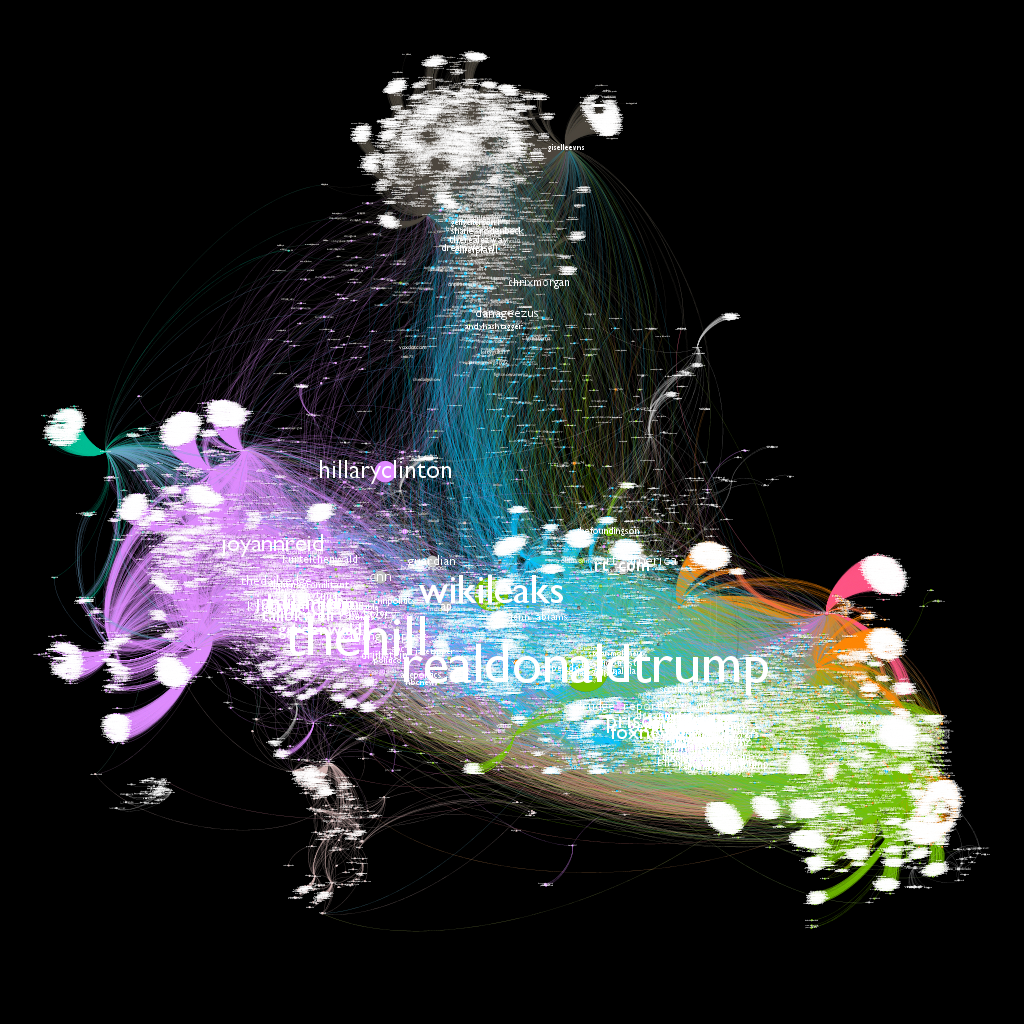
\includegraphics[width=0.95\linewidth]{Network_modularity.png}
\caption[Retweet network]{The entire retweet network. Nodes represent profiles, while a connection represents at least one retweet between them. Node and label size represent popularity (indegree). Colors represent the communities detected by the Louvain algorithm.}
\label{fig:graph}
\end{figure}


\subsection{Findings}

We run a modularity-based community detection, following the Louvain Method (\cite{blondel_fast_2008}). Figure~\ref{fig:distcom} shows the distribution of algorithm communities among the qualitative account categories created by Linvill/Warren (\cite*{linvill_troll_2018}). For further analysis, we want to rely on communities that were computed with the Louvain Method, since they originate from the structure of ties within our dataset and this appears to be more consistent with the overall method of SNA. To not exceed the scope of this paper, we narrow down our analysis by merging all minor communities below an arbitrary threshold of 50 nodes, since they presumably bear more risk of yielding unrepresentative findings. We then apply the qualitative categorization to our newly distincted communities. In Figure~\ref{fig:distcom}, we see that some categories overlap strongly with distinct communities, whereas other categories show a rather mixed composition in our data. 94\% of the left troll category is captured with one community, which will be our new left troll community. The hashtager community is 90\% captured by one community, which will be our new hashtager troll community. 90\% of the right troll category consist of two major communities with shares of 52\% and 38\%, which we merge to one new right troll community. We justify this merger by arguing that these two communities could represent distinct right-wing groups underneath a general right-wing community (e.g. Conspiracy Theorist vs. Alt Right User). (\cite{kaiser_unite_2018}).  We argue, that for these categories, which are overlapping with at least 90\%, there is sufficient congruence to continue using the qualitative attributes. The non-english troll category consists of multiple communities, with a biggest community share of 27\%. Non of the non-english or other categories passes our threshold community size of 50, which leaves us with four distinct communities: \textit{Right Troll}, \textit{Left Troll}, \textit{Hashtager} and \textit{Other}. It is important to note, that by using this set of communities, we are treating some nodes as e.g. right trolls, even though they have been categorized as left trolls by Linvill/Warren (\cite*{linvill_troll_2018}). This bears the risk of having biased results. Though, with the given incongruence of the account categorization with our detected communities, having some potential bias appears inevitable. In Figure~\ref{fig:distcat}, the distribution of account categories among our new communities is depicted, which illustrates this potential bias.

\begin{figure}[!ht]
\centering
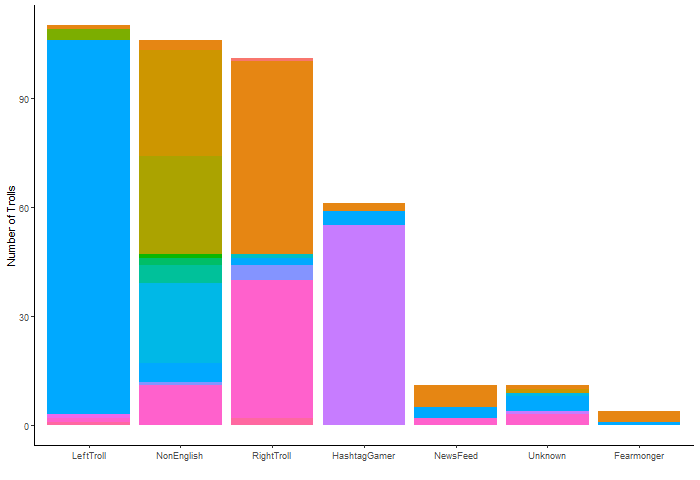
\includegraphics[width=0.95\linewidth]{final_figure1.png}% die Breite des eingefügten Bildes entspricht 95% einer Zeilenlänge
\caption[Distribution of account categories in communities]{Distribution of account categories by Linvill and Warren. Color reflects account categories among communities detected by the Louvain Method.}
\label{fig:distcom}
\end{figure}

\begin{figure}[!ht]
\centering
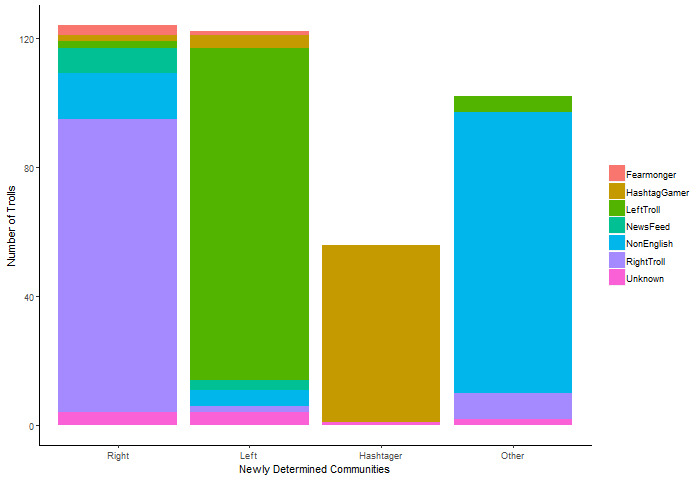
\includegraphics[width=0.95\linewidth]{final_figure2.png}% die Breite des eingefügten Bildes entspricht 95% einer Zeilenlänge
\caption[Distribution of communities in account categories]{Distribution of account categories among communities detected by the Louvain Method. Color reflects account categories by Linvill and Warren.}
\label{fig:distcat}
\end{figure}

Next, the graph densities are calculated for the subgraphs of our newly determined communities. Figure~\ref{fig:dens} shows the graph densities for the three communities for both directed and undirected versions of each subgraph. As a mode for creating an undirected graph from a directed one, we chose too keep a tie for every relationship that is only defined with a single directional tie, but also to collapse all reciprocal ties into one tie in the undirected graph. This avoids having multiple ties in one relationship. First of all, we see that the undirected subgraphs' densities are approximately twice as high as directed ones, with only minor deficits. With our mode of creating an undirected graph, we can interpret this that way, that there are not many reciprocal ties in the subgraphs. If there was a considerable amount of reciprocal ties, they would cause a higher density of the directed subgraph in comparison to the undirected one (>50\%).

\begin{figure}[!ht]
\centering
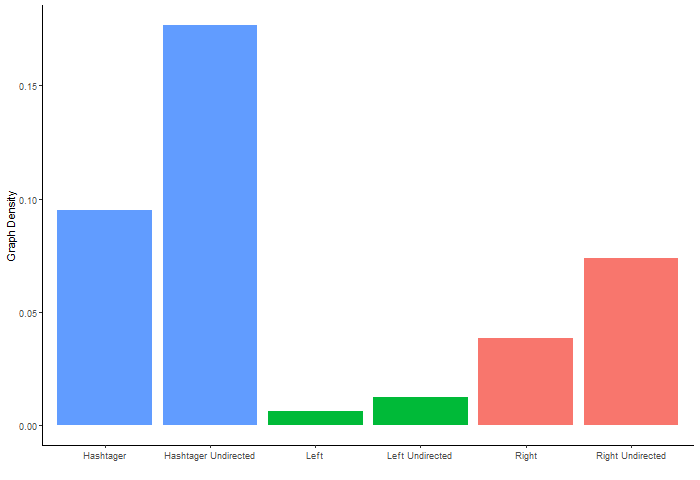
\includegraphics[width=0.95\linewidth]{final_figure3.png}
\caption[Graph densities]{Graph densities in the three biggest communities.}
\label{fig:dens}
\end{figure}

Examining the magnitude of densities across different community subgraphs, we find that the hashtager community is the most dense by a significant margin. Approximately 17.7\% of all possible ties are present for the undirected subgraph. This could relate to the nature of this community. As laid out above, hashtag gamers retweet themselves playing a word game, which means that it appears to constitute this community's cohesion to retweet one another frequently. Right trolls have the second largest density with 7.4\%, which is more than six times larger than the left community's density of 1.2\%, looking at the numbers for the undirected graphs.

We now  analyze the degree centrality of our graph. We start with the outdegree, which we use as a measure for centrality and the weighted outdegree, which gives additional information on the activity of the user. Because of our network is ego-centered around the central group of trolls, only troll accounts have outdegrees. Table~\ref{tab:out} shows the top 10 users ranked by outdegree.

\begin{table}[!ht] \centering 
\begin{tabular*}{.95\linewidth}{@{\extracolsep{\fill}} lrrrrr} 
\\[-1.8ex]\hline 
\hline \\[-1.8ex] 
User & Community & Category & Followers & \( d_{out}(n_{i}) \) & \( d_{out}(n_{i}) \) weighted \\ 
\hline \\[-1.8ex] 
ameliebaldwin & Other & RightTroll & $2,464$ & $4,896$ & $9,243$ \\ 
patriotblake & Other & RightTroll & $2,035$ & $2,856$ & $4,106$ \\ 
hyddrox & Right & RightTroll & $2,225$ & $2,650$ & $6,788$ \\ 
giselleevns & Hashtager & Unknown & $24,344$ & $2,282$ & $5,403$ \\ 
cookncooks & Other & RightTroll & $1,468$ & $2,153$ & $2,893$ \\ 
emileewaren & Other & RightTroll & $1,909$ & $2,116$ & $2,891$ \\ 
dorothiebell & Right & RightTroll & $1,893$ & $2,010$ & $2,874$ \\ 
baobaeham & Left & LeftTroll & $1,032$ & $1,802$ & $3,215$ \\ 
michellearry & Right & RightTroll & $3,229$ & $1,611$ & $2,677$ \\ 
\_nickluna\_ & Right & RightTroll & $1,457$ & $1,597$ & $2,825$ \\ 
\hline \\[-1.8ex] 
\end{tabular*} 
  \caption[Outdegree]{Top 10 users ranked by outdegree} 
  \label{tab:out} 
\end{table}  

The first ranked user \textit{ameliebaldwin} sticks out with an outdegree of 4,896, meaning that the user retweeted nearly 5,000 different users. The weighted outdegree of \textit{ameliebaldwin} is 9,243, which includes multiple retweets of the same user. Since the weighted outdegree is significantly higher than the unweighted one, this means that \textit{ameliebaldwin} retweeted a large number of users only a few times, rather than retweeting the same small number of users over and over again. The category and community allocation disagree for \textit{ameliebaldwin}. While the qualitative analysis by Linvill/Warren \cite*{linvill_troll_2018} found the user to be a right troll, the community detection algorithm did not find it to belong one of the major right troll communities. This exact pattern of disagreement reappears for three other users in Table~\ref{tab:out}. Subsequent to \textit{ameliebaldwin}, there is a group of accounts retweeting more than 2,000 different users, which is mainly dominated by right trolls following the categorization, but also with partial disagreement, following the above-mentioned pattern. The fourth ranked user \textit{giselleevns} sticks out for having the most followers in the ranking with 24,344. With a mean number of followers of 3,022 and a maximum of 61,109, \textit{giselleevns} appears to be one of the most followed accounts in the dataset. Though, it needs to be noted, that information on followers is only available for troll accounts in our dataset. Contrary to the mostly right troll dominated top ten ranked outdegree users, \textit{giselleevns} was allocated to the hashtager community, with disagreement of Linvill/Warren \cite*{linvill_troll_2018}, who could not attribute the account to a category. When ranking the account for weighted outdegree, as can be seen in Table~\ref{tab:wout}, the picture slightly changes. While some accounts like \textit{ameliebaldwin} and \textit{giselleevns} remain in high-ranked positions, six left troll accounts are now in the ranking, for which category and community allocation mostly agrees.

\begin{table}[!ht] \centering 
\begin{tabular*}{.95\linewidth}{@{\extracolsep{\fill}} lrrrrr} 
\\[-1.8ex]\hline 
\hline \\[-1.8ex] 
User & Community & Category & Followers & \( d_{out}(n_{i}) \) & \( d_{out}(n_{i}) \) weighted \\ 
\hline \\[-1.8ex] 
ameliebaldwin & Other & RightTroll & $2,464$ & $4,896$ & $9,243$ \\ 
hyddrox & Right & RightTroll & $2,225$ & $2,650$ & $6,788$ \\ 
giselleevns & Hashtager & Unknown & $24,344$ & $2,282$ & $5,403$ \\ 
patriotblake & Other & RightTroll & $2,035$ & $2,856$ & $4,106$ \\ 
mrclydepratt & Left & LeftTroll & $914$ & $1,583$ & $3,262$ \\ 
brianaregland & Other & LeftTroll & $768$ & $1,360$ & $3,259$ \\ 
baobaeham & Left & LeftTroll & $1,032$ & $1,802$ & $3,215$ \\ 
datwisenigga & Left & LeftTroll & $904$ & $1,540$ & $3,196$ \\ 
willisbonnerr & Left & LeftTroll & $571$ & $1,563$ & $3,155$ \\ 
melanymelanin & Left & LeftTroll & $963$ & $1,079$ & $3,071$ \\ 
\hline \\[-1.8ex] 
\end{tabular*} 
  \caption[Outdegree weighted]{Top 10 users ranked by weighted outdegree} 
  \label{tab:wout} 
\end{table} 

The highest ranked left troll account \textit{mrclydepratt} has a weighted outdegree of 3,262 and an unweighted one of 914. Compared to the top ranked presumably right troll accounts, the left troll accounts approximately only have a maximum of half of the unweighted outdegree, but are much closer on the weighted outdegree. This means that the left trolls retweet a smaller number of accounts more often than right trolls do. This relates to the lower graph density for the left troll community that was computed above.

When examining the accounts with the highest indegrees, contrary to outdegree, both trolls and non-troll accounts are included. We use indegree as a measure for prestige, as it shows how often a user is chosen to be retweeted by the trolls. Table~\ref{tab:in} shows the ten highest ranked accounts for unweighted indegree. Here, mostly non-troll accounts are present. Among them, we find  accounts from popular U.S. politicians like Donald Trump or Hillary Clinton, but also accounts of official media outlets like The Hill or Fox News. The account \textit{thehill} has the highest unweighted indegree with 102, which represents the number of unique trolls who retweeted him in the data. The indegree quickly declines from 102 for rank one to 53 for rank ten. One account that sticks out is \textit{ten\_gop}, who is the only troll among the ten highest indegrees. He is categorized a right troll by both Linvill/Warren \cite*{linvill_troll_2018} and the community detection algorithm. Further investigation shows that \textit{ten\_gop} pretended to be an official Republican Party account, which fits his ranking among the other official accounts. %% Page 15: https://assets.documentcloud.org/documents/4380502/Indictment.pdf%%

\begin{table}[!ht] \centering 
  \begin{tabular*}{.95\linewidth}{@{\extracolsep{\fill}} lrrrr} 
\\[-1.8ex]\hline 
\hline \\[-1.8ex] 
User & Community & Category & \( d_{in}(n_{i}) \) & \( d_{in}(n_{i}) \) weighted \\ 
\hline \\[-1.8ex] 
thehill & Non-Troll & Non-Troll & $102$ & $358$ \\ 
realdonaldtrump & Non-Troll & Non-Troll & $100$ & $544$ \\ 
wikileaks & Non-Troll & Non-Troll & $82$ & $247$ \\ 
blicqer & Non-Troll & Non-Troll & $69$ & $2,207$ \\ 
hillaryclinton & Non-Troll & Non-Troll & $61$ & $98$ \\ 
joyannreid & Non-Troll & Non-Troll & $58$ & $267$ \\ 
prisonplanet & Non-Troll & Non-Troll & $56$ & $462$ \\ 
jamilsmith & Non-Troll & Non-Troll & $55$ & $118$ \\ 
ten\_gop & Right & RightTroll & $53$ & $430$ \\ 
foxnews & Non-Troll & Non-Troll & $53$ & $336$ \\ 
\hline \\[-1.8ex] 
\end{tabular*} 
\caption[Indegree]{Top 10 users ranked by indegree} 
  \label{tab:in} 
\end{table} 

Table~\ref{tab:win} shows the top ten ranked accounts for weighted indegree. Similarly to unweighted indegree, official politician or news outlet accounts dominate the picture. Weighted indegree appears to not correlate strongly with the unweighted indegree for the top ten ranked accounts, wherefore the order changed substantially. Four new accounts appear in the ranking compared to Table~\ref{tab:in}. These accounts have a relatively low number of trolls retweeting them, but in a relatively high frequency. For example, the second ranked user \textit{conservatexian} has only 30 different users retweeting him 1,082 times, which results in an average of ca 37 retweets per troll. For the account \textit{nine\_oh} the average is even higher, with ca 45 retweets per troll. For comparison, \textit{realdonaldtrump} has an average of ca 5 and the only right troll in the ranking \textit{ten\_gop} a average of ca 8.

\begin{table}[!ht] \centering 
  \begin{tabular*}{.95\linewidth}{@{\extracolsep{\fill}} lrrrr} 
\\[-1.8ex]\hline 
\hline \\[-1.8ex] 
User & Community & Category & \( d_{in}(n_{i}) \) & \( d_{in}(n_{i}) \) weighted \\ 
\hline \\[-1.8ex] 
blicqer & Non-Troll & Non-Troll & $69$ & $2,207$ \\ 
conservatexian & Non-Troll & Non-Troll & $30$ & $1,082$ \\ 
realdonaldtrump & Non-Troll & Non-Troll & $100$ & $544$ \\ 
nine\_oh & Non-Troll & Non-Troll & $11$ & $500$ \\ 
prisonplanet & Non-Troll & Non-Troll & $56$ & $462$ \\ 
zaibatsunews & Non-Troll & Non-Troll & $16$ & $451$ \\ 
gerfingerpoken & Non-Troll & Non-Troll & $46$ & $434$ \\ 
ten\_gop & Right & RightTroll & $53$ & $430$ \\ 
bizpacreview & Non-Troll & Non-Troll & $17$ & $401$ \\ 
beforeitsnews & Non-Troll & Non-Troll & $8$ & $399$ \\ 
\hline \\[-1.8ex] 
\end{tabular*} 
\caption[Indegree weighted]{Top 10 Users ranked by Weighted Indegree} 
  \label{tab:win} 
\end{table}

For the k-core we limited the network to the core of \( \text{ k } = 10 \), for the k-in-core to \( \text{ k-in } = 4 \), meaning that the users of the k-10-core have been retweeted and/or retweet others at least 10 times and the users of the k-4-in-core have been retweeted at least 4 times, which is the maximum value for k-in in the dataset.\footnote{We disregarded self loops, since they cannot count as new information and are therefore irrelevant for analyzing information spreading.} The original graph consists of 36,889 nodes with 147,428 edges, of which the k-10-core contains 1257 (3.4\%) nodes and 18214 (12.3\%) edges, and the k-in-4-core 1754 (4.8\%) nodes and 11988 (8.1\%) edges respectively. Although the k-in-4-core contains some nodes more, it has far less edges, which is shown in Figure~\ref{fig:kcore}, that depicts both subgraphs. It is immediately apparent, that the k-core still contains the basic structure of the network with its three main clusters, while the k-in-core only consists of one large cluster with mainly right-wing accounts and one very small hashtager cluster. This is contingent with the findings regarding degree centrality, which showed that the right-wing trolls have a larger unweighted indegree, while the results are more equal for the unweighted degree. This is no surprise considering the k-in-core is calculated through the indegree. Interestingly, the k-10-core looks very different.\footnote{A quick analysis in Gephi via filtering gives one cluster as a result only for the k-18-core, when 271 nodes are left.} Here, the basic structure of the entire network is still intact, which indicates a lot of left and hashtager accounts retweeting right-wing IRA accounts in the k-10-core. Otherwise, we would see more of the former in the k-in-core, but as they only have a large outdegree (because of retweeting relatively more right-wing accounts) the two subgraphs are structured this way. In other words, IRA accounts retweet other trolls mainly from the left and hashtager clusters, while right-wing accounts mainly retweet themselves.

\begin{figure}[!ht]
\centering
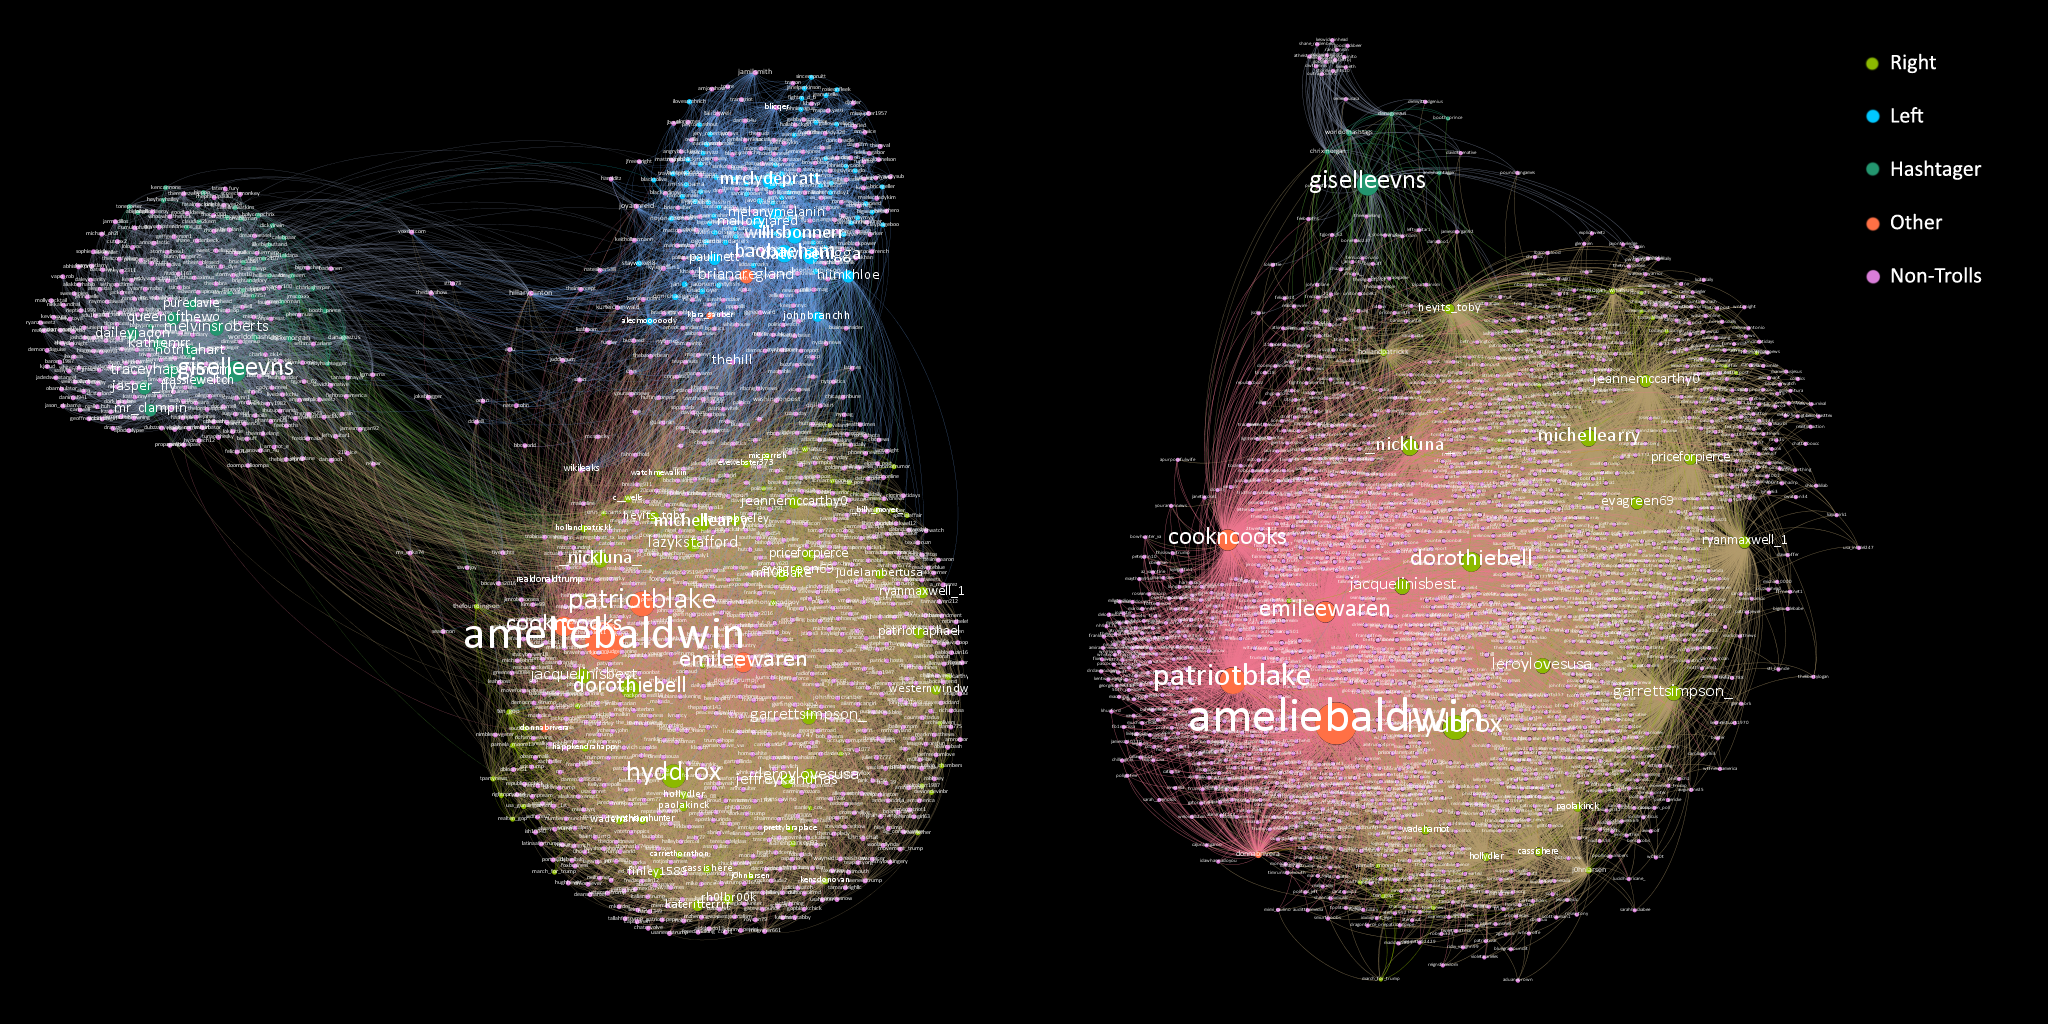
\includegraphics[width=0.95\linewidth]{final_k_graphs.png}
\caption[k-core and k-in-core]{k-10-core and k-in-4-core. Node and label size represent outdegree centrality, colors reflect community.}
\label{fig:kcore}
\end{figure}

Since the k-in-core consists mostly of right-wing accounts, a further analysis of the k-10-core seems to be more fruitful. The accounts in the k-10-core are those with the best positions in the network regarding the ability to spread information. We therefore proceed to examine the most active accounts, since they can be considered as the most influential. Figure~\ref{fig:k10in} provides an overview of the 30 accounts with the highest outdegree within the k-10-core, and thus the profiles who retweeted the relevant accounts most often. The profile \textit{ameliebaldwin} has by far the largest outdegree, which puts this account at the central position of the core. Interestingly, of the top 6 profiles, 4 were categorized as \textit{Other} by the community detection algorithm. Looking on Figure~\ref{fig:kcore}, they all are very close to the right-wing community (the same is true for the k-in-core). Linvill and Warren categorized most of them as right-wing as well, which indicates some inaccuracy of the community detection algorithm, i.e. it is to sharp, thus detecting too many communities. Seeing them as right-wing shows a very clear dominance of right-wing profiles concerning information super-spreaders, which is consistent with the our previous findings.

\begin{figure}[!ht]
\centering
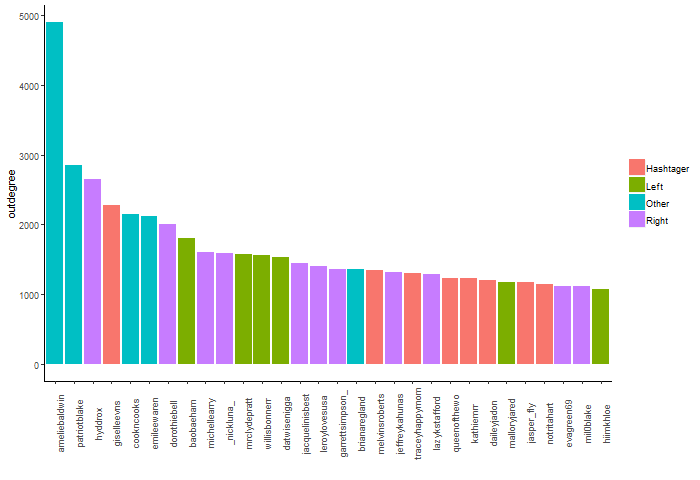
\includegraphics[width=0.95\linewidth]{k10_figure}
\caption[Outdegree in the k-core]{Top 30 user regarding outdegree in the k-10-core.}
\label{fig:k10in}
\end{figure}


\subsection{Discussion}

Our analysis shows that the IRA did not only conduct astroturfing for one single community, but for at least three distinct social groups on Twitter. Targeting all of them ensured a way broader influence, especially considering the selection of left- and right-wing communities, suggesting a strategy to enhance an already present divide in society, that is reflected on Twitter. We can therefore verify Linvill and Warren's qualitative findings out of the structure of the network itself. The community detection results in a distribution of the right-wing cluster into two smaller communities. We can only speculate this being due to the right-wing's division into subgroups e.g. conservatives and alt-right. Another possibility is the relatively small size or the ego-centered character of our network leading to a too fine result of the algorithm. An interesting finding is the IRA's targeting of the \textit{Hashtag Gamer} community, since they are not known for their wide political influence. Again, we can only speculate: Since they are a relatively well connected group, therefore information can be spread well through their channels. Adding Linvill and Warren's findings, the IRA might have tried to politicize this group to widen the scope of their astroturfing to a big, well-connected, but not very politically active twitter community.

Comparing the three communities, the IRA put a definite focus on the right-wing community. Right troll accounts are retweeting more regarding the mere quantity, as well as the range of different accounts retweeting. Accounts in the left community are less well connected and tend to repeatedly retweet the same accounts very often. It is unclear, weather this is intentional IRA behavior or is based in the way those communities function differently in the way they interact within, although we can assume that it is in fact intentional, since knowing from the statements of Lyudmila Savchuk (\cite{savchuk_inside_2018}), an investigative journalist who worked for a couple of months undercover for the IRA, that every tweet was seen through before posting. The \textit{Hashtag Gamers} are the most connected community, but this is most likely due to the nature of the hashtag-games this community is engaged in.

The IRA's focus on the right-wing community is reinforced through those accounts mainly retweeting themselves, while user from the other communities do retweet right-wing accounts. Again, we can only assume, this is intentional and not based in the community structure. Weather intentional or not, the IRA was definitely more active and able to spread information broader within and from the right-wing community. The analysis of the k-10-core and the k-in-4-core locates the super-spreaders of information mostly in the right-wing community as well, which is no surprise considering the fact that this community is retweeted by everyone else. The most active troll account in the most connected core of the network is by far \textit{ameliebaldwin}. It is unclear why exactly this account has such a key position, while the other super-spreaders are relatively close to each other, which suggests a division of labor between a couple of accounts. Although the focus is on the right-wing community, left-wing and \textit{Hastag Gamer} accounts are not unimportant, some of them occupying considerable central positions, just in total in a lesser degree than right-wing trolls.

The most prestigious accounts, meaning the accounts retweeted by the most trolls, range from accounts of important politicians like President Trump or Hillary Clinton through big news channels like The Hill or Fox News to political journalists like Joy Reid or Jamil Smith. This makes sense, since those profiles have a lot of followers and people are referring on them very often. This would suggest those profiles also being the most prestigious quantitatively, however with the exception of President Trump other profiles take their spot. With \textit{blicqer} a black activist user is by far the most retweeted profile in our dataset, the second being \textit{conservatexian}, a right-wing user, who stand as prime examples for users of the left and right communities. Both are big profiles, but not of official government or news accounts. It suggests that the IRA rather shares information from unofficial accounts which do not employ standards regarding information checking before they tweet.

This study had to deal with some severe limitations regarding the available data, the network being ego-centered being the main obstacle, since it allows for less interpretation. While we have a lot of information on the trolls' own retweet behaviour, we do not know which troll has been retweeted how much by non-troll users. This left us with fewer possibilities than with a complete non-ego-centered network (e.g. the number of regular tweets of accounts as a node attribute or ratios of how many retweets per tweet a user is receiving can enhance the analysis). We cannot presume that the indegree of a troll account is a good heuristic for the actual number of retweets an account gets, since non-troll retweet behavior could be completely different from troll activity on Twitter. It is important to highlight, that a complete network of the same nodes would presumably change the structure of the graph, including centralities and community allocation. This implies, that our graph does not tell us the actual positions of the nodes in the holistic Twitter network. With a bigger and thus more representative dataset, the smaller communities of trolls we categorized as other would be represented accurately and could be analyzed. Our graph mainly is a depiction of how the group of trolls constituting our dataset interacted with each other and whose tweets they chose to spread. Outdegree centralities and the k-core measure are therefore eligible to compare trolls or groups of trolls with each other. This is why our findings on interaction or cooperation between the trolls should be valid within the scope of an ego-centered network, although we rely on the assumption that there is no substantial group of trolls missing, which would skew the results comparing the communities.


\section{Conclusion}

Distinguishing true from false information becomes increasingly difficult in today's social media landscape. In this paper, we try to shed some light on the structure and strategy of the organized disinformation campaign of the IRA. Situating their behavior in astroturfing as a strategy for agenda building, we showed how they target specific communities on Twitter, in order to create the impression of a certain public opinion as diametrical opposed. We have explored the division of labor of different troll accounts, as well as their positions within a retweet network. Instead of creating the impression of one social movement, the IRA is operating within different, even opposed communities, while focusing on the right-wing community. With one exception, they have a couple of accounts in central positions spreading mainly (dis-)information regarding political topics. Hence, we can confirm, that the problem of disinformation campaigns cannot be solved, only marginal, improved, by banning some highly influential accounts, even if examples like \textit{ten\_gop} might suggest otherwise. Interestingly, our results show the IRA trying to influence the well connected, but not distinct political community of \textit{Hashtag Gamers}, which calls for attention. If organizations like the IRA specifically target non-political communities, the problem of agenda-building through disinformation campaigns is even bigger than assumed right now.

Although the dataset used in this paper posed some severe limitations -- especially the dataset consisting of only tweets from the troll accounts, which resulted in the network being ego-centered, as well as it not being complete -- we were able to highlight central aspects of the strategies of the IRA. Thus, we demonstrated the merits of SNA in exploring strategies of organizations conducting disinformation campaigns, while having no possibility to learn of their intentions through other social science methods like interviews. SNA's methodological approach in taking structures as a starting point make it the prime tool for cases like this, even if the data is incomplete. That being said, to fully understand how organizations like the IRA work, much more research is needed. Especially with a more complete dataset, that does not result in just a retweet network, a SNA can deliver more valid results. This study pointed to some further questions regarding the functioning of communities on Twitter. Here, more sociological knowledge can help identifying weather the IRA's different retweet structure in different communities is strategic or rooted in those communities themselves, e.g. through an analysis of different trending hashtag discussions, which could shed light on how specific community behavior might change between policy areas. The question why some troll accounts have much more output also should be discussed. Lastly, it can be learned a lot from comparing cases. Astroturfing is no new phenomenon, accordingly compare the IRA with similar agencies can give a better understanding of how these operate. Taking one step back, SNA does not necessarily have to be conducted via a network of retweets, but could also be done with mentions.\footnote{Mentions mean the tagging of another user's name without spreading information of their tweet.} Contrary to retweets, mentions appear to be more easily used to contradict another user, which would make the ties a lot harder to define and interpret, but an interesting choice for comparing a network drawn from the same data.

All in all, influencing and agenda-building poses a big problem, especially for democratic states, since social media here reaches very far into society. Right now organizations like the IRA have the advantage, because they were able to operate out of the dark. But through in-depth research happening right now, of which this paper is only a marginal part, we can analyze their structure and strategies and thus hopefully find the necessary tools to prevent disinformation campaigns from reaching considerable impact.


\newpage

\printbibliography


\end{document}
